% Options for packages loaded elsewhere
\PassOptionsToPackage{unicode}{hyperref}
\PassOptionsToPackage{hyphens}{url}
\documentclass[
  10pt,
]{article}
\usepackage{xcolor}
\usepackage[margin=20mm]{geometry}
\usepackage{amsmath,amssymb}
\setcounter{secnumdepth}{-\maxdimen} % remove section numbering
\usepackage{iftex}
\ifPDFTeX
  \usepackage[T1]{fontenc}
  \usepackage[utf8]{inputenc}
  \usepackage{textcomp} % provide euro and other symbols
\else % if luatex or xetex
  \usepackage{unicode-math} % this also loads fontspec
  \defaultfontfeatures{Scale=MatchLowercase}
  \defaultfontfeatures[\rmfamily]{Ligatures=TeX,Scale=1}
\fi
\usepackage{lmodern}
\ifPDFTeX\else
  % xetex/luatex font selection
\fi
% Use upquote if available, for straight quotes in verbatim environments
\IfFileExists{upquote.sty}{\usepackage{upquote}}{}
\IfFileExists{microtype.sty}{% use microtype if available
  \usepackage[]{microtype}
  \UseMicrotypeSet[protrusion]{basicmath} % disable protrusion for tt fonts
}{}
\makeatletter
\@ifundefined{KOMAClassName}{% if non-KOMA class
  \IfFileExists{parskip.sty}{%
    \usepackage{parskip}
  }{% else
    \setlength{\parindent}{0pt}
    \setlength{\parskip}{6pt plus 2pt minus 1pt}}
}{% if KOMA class
  \KOMAoptions{parskip=half}}
\makeatother
\usepackage{longtable,booktabs,array}
\usepackage{calc} % for calculating minipage widths
% Correct order of tables after \paragraph or \subparagraph
\usepackage{etoolbox}
\makeatletter
\patchcmd\longtable{\par}{\if@noskipsec\mbox{}\fi\par}{}{}
\makeatother
% Allow footnotes in longtable head/foot
\IfFileExists{footnotehyper.sty}{\usepackage{footnotehyper}}{\usepackage{footnote}}
\makesavenoteenv{longtable}
\usepackage{graphicx}
\makeatletter
\newsavebox\pandoc@box
\newcommand*\pandocbounded[1]{% scales image to fit in text height/width
  \sbox\pandoc@box{#1}%
  \Gscale@div\@tempa{\textheight}{\dimexpr\ht\pandoc@box+\dp\pandoc@box\relax}%
  \Gscale@div\@tempb{\linewidth}{\wd\pandoc@box}%
  \ifdim\@tempb\p@<\@tempa\p@\let\@tempa\@tempb\fi% select the smaller of both
  \ifdim\@tempa\p@<\p@\scalebox{\@tempa}{\usebox\pandoc@box}%
  \else\usebox{\pandoc@box}%
  \fi%
}
% Set default figure placement to htbp
\def\fps@figure{htbp}
\makeatother
\setlength{\emergencystretch}{3em} % prevent overfull lines
\providecommand{\tightlist}{%
  \setlength{\itemsep}{0pt}\setlength{\parskip}{0pt}}
\usepackage{fontspec}
\usepackage{xeCJK}
\setCJKmainfont{Microsoft YaHei}
\setmainfont{TeX Gyre Termes}
\usepackage{tikz,pgfplots}
\pgfplotsset{compat=1.18}
\usepackage{float}
\let\origfigure\figure
\let\endorigfigure\endfigure
\renewenvironment{figure}[1][]{\origfigure[H]}{\endorigfigure}
\usepackage{graphicx}
\setlength{\emergencystretch}{3em}
\usepackage{fancyhdr}
\pagestyle{fancy}
\fancyhf{}
\fancyfoot[C]{\thepage}
\renewcommand{\headrulewidth}{0pt}
\usepackage{bookmark}
\IfFileExists{xurl.sty}{\usepackage{xurl}}{} % add URL line breaks if available
\urlstyle{same}
\hypersetup{
  hidelinks,
  pdfcreator={LaTeX via pandoc}}

\author{}
\date{}

\begin{document}

\section{第九阶段报告：图像对齐、分数阈值与细胞核中心检测}\label{ux7b2cux4e5dux9636ux6bb5ux62a5ux544aux56feux50cfux5bf9ux9f50ux5206ux6570ux9608ux503cux4e0eux7ec6ux80deux6838ux4e2dux5fc3ux68c0ux6d4b}

2026 年 11 月 18---20
日。本阶段最清晰的发现是：对齐依赖与预测分数偏低是两种不同的失效方式。全部编码层参与适配的检测器，主要从多种对齐的预测位置汇总中获益；加入平移训练的检测器，则在原来采用的阈值以下定位到了大量细胞核。新完成的固定诊断逐核区分了这些情况。

本文覆盖有研究价值的完整证据链：早期的平移训练（P15）、全层适配（P22）、中间分数图与插值诊断（D32、D33）、位置读出（P34）、十六种对齐的分数图汇总（P35）、阈值选择与预测点一致性汇总（P36），以及本次新增的保存点诊断（D37）。D32、D33用于交代背景，P34至D37构成本阶段的主体。

P36八个模型均完成科学计算。七个数组任务正常结束；平移训练种子19在计算结束后的保存步骤失败，单独保存任务55895127已成功补齐。八份回收收据通过，242个已回收文件与原保存摘要一致；成对判定与原分析全部复算一致。D37在分解漏检前，逐图重现了三种解码的全部计数。P34全层种子1的部分输出仍保留，尚无完整评估结果。

\newpage

\section{检测器、图像与统计口径}\label{ux68c0ux6d4bux5668ux56feux50cfux4e0eux7edfux8ba1ux53e3ux5f84}

八个检测器均使用130轮训练后的最后检查点。P22对照仅更新最后12个编码层，实验模型更新全部24层；P15对照为其自身的最后12层模型，实验模型训练时加入每轴最多16像素的整数平移。每项配置均有种子19和1。P15与P22的对照来自不同训练过程，各自沿用本轮的成对比较。

数据沿用fold
1内部的训练与开发评估划分：训练图像2134张，开发评估图像522张。P36按图像编号散列固定抽取240张训练图像，含5581个标注核；开发评估图像含12250个标注核，其中145个为不接触图像边界的死亡细胞核。死亡类包括凋亡和坏死细胞核。中心区域分析使用7014个距四边至少24像素、在十六种对齐下都可见的开发评估核。

预测点距标注中心不超过三像素，并经最大匹配数的一对一分配，才记为匹配。每轴平移−8、−4、0、4像素，共十六种；空出区域分别采用白色和镜像填充，预测点移回原坐标。阈值与一致性规则只在平移后的训练图像上选择，在读取开发评估图像前写入磁盘；原对齐不参与选择。

检出率指被匹配的标注核比例，精度指能匹配标注的预测点比例，F1是两者的调和平均。本文为CPU单精度的核中心检测结果，原BF16记录单独保留。同一个核的十六种对齐是重复观察；进入实例分割评估后，继续采用最后检查点、官方指标实现与三折报告。

\newpage

\section{位置读出与分数图平均：此前实验解决了什么问题}\label{ux4f4dux7f6eux8bfbux51faux4e0eux5206ux6570ux56feux5e73ux5747ux6b64ux524dux5b9eux9a8cux89e3ux51b3ux4e86ux4ec0ux4e48ux95eeux9898}

P34保持检测器冻结，训练73986参数的位置读出。三个任务完成；第四个在第二个读出首轮用时1400.3秒、超过1300秒保护上限后停止，全层两种子的最终比较尚不完整。

在48张选定训练图像上，读出误差不超过三像素的核占99.4\%---99.8\%；在开发评估图像上，随读出与检测器不同为70.6\%---80.6\%。移动并合并预测点，为三个检测器分别新增158、172、172个匹配，同时丢失173、182、158个。读出自身的位置误差足以抵消大部分新增匹配。加入平移训练改善了读出在平移图像上的定位，但最终检测净变化仍很小。

更有价值的是检测器对照：原训练图像检出率96.0\%---98.2\%，同样图像移动(5,3)像素后降至56.1\%---64.6\%。P35把这一比较扩展到十六种对齐。中心区域训练核的原对齐检出率为97.4\%---99.2\%，其余十五种仅67.1\%---72.6\%；开发评估图像原对齐与其他对齐都在约61\%---68\%。

P35发现86\%---89\%的中心区域开发评估核至少在一种对齐下匹配，51\%---61\%只在部分对齐下匹配。直接平均细窄、位置不同的分数峰，在阈值0.5下只匹配9\%---15\%的开发评估核，精度95\%---96\%。峰的位置变化与平均后的分数下降，促使后续分别研究预测位置汇总和阈值。

\begin{center}
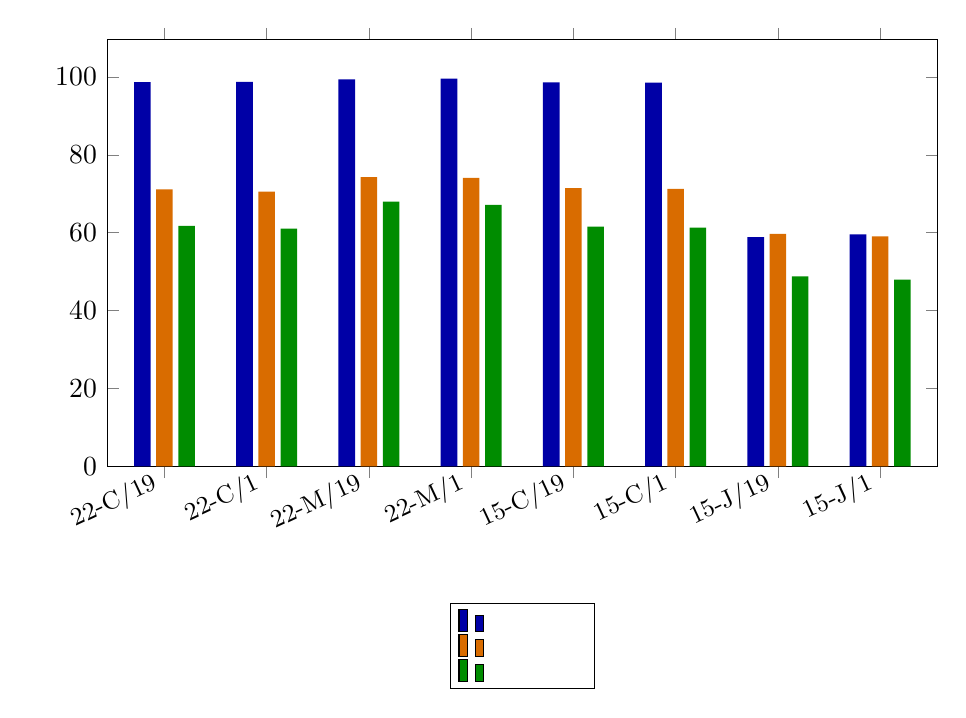
\begin{tikzpicture}
\begin{axis}[width=\linewidth,height=7cm,ymin=0,xtick={0,1,2,3,4,5,6,7},xticklabels={22-C/19,22-C/1,22-M/19,22-M/1,15-C/19,15-C/1,15-J/19,15-J/1},x tick label style={font=\small,rotate=25,anchor=east},ylabel={匹配率（百分比）},legend style={at={(0.5,-0.32)},anchor=north,legend columns=1,font=\small},enlarge x limits=0.08,ybar,bar width=6pt]
\addplot[fill=blue!65!black,draw=none] coordinates {(0,98.654846) (1,98.715989) (2,99.388566) (3,99.602568) (4,98.593702) (5,98.563131) (6,58.850504) (7,59.584225)};
\addplot[fill=orange!85!black,draw=none] coordinates {(0,71.150515) (1,70.537043) (2,74.285132) (3,74.103740) (4,71.478651) (5,71.282992) (6,59.702436) (7,59.082849)};
\addplot[fill=green!55!black,draw=none] coordinates {(0,61.777398) (1,61.091151) (2,67.968824) (3,67.191332) (4,61.573044) (5,61.304059) (6,48.817603) (7,47.957418)};
\legend{训练图像原对齐,训练图像其余十五种对齐,开发评估图像其余十五种对齐}
\end{axis}
\end{tikzpicture}
\end{center}

P36在240张训练图像上重复了对齐比较。22-C、22-M、15-C、15-J分别表示前文定义的四项配置，后缀为种子；统计限于中心区域核，使用镜像填充。

\newpage

\section{训练集选择的阈值找回了低分数细胞核}\label{ux8badux7ec3ux96c6ux9009ux62e9ux7684ux9608ux503cux627eux56deux4e86ux4f4eux5206ux6570ux7ec6ux80deux6838}

各最后12层对照与全层种子19选定阈值0.3，全层种子1选0.4，两个平移训练模型均选0.2。这些阈值根据平移后训练图像的全部标注核F1选择，两种填充合并统计。

平移训练模型的变化最明显。阈值0.5下，两种子分别匹配4771、4600个开发评估核，精度86.57\%、86.38\%，内部死亡核均为44个。改用训练集选定的0.2后，匹配8463、8542个，精度66.04\%、66.50\%，内部死亡核101、99个。保存点重放确认，新增3692、3942个匹配，原匹配没有丢失，同时新增了大量无法匹配标注的预测点。

全层模型降低阈值后分别新增293、145个匹配，各多两个内部死亡核；F1仅提高0.0034、0.0015。平移训练模型与对照需要不同的分数解释。早期P15在固定0.5下的判定仍属于原配置的历史记录，本次检验的是另一个明确在训练集上选择的解码。

平移训练模型在训练图像上用于选择阈值的F1约0.795、0.796，在开发评估图像上为0.675、0.681。平移训练减小了原对齐的特殊优势，训练与开发评估之间仍有明显差距。

\begin{longtable}[]{@{}lrrrrrr@{}}
\toprule\noalign{}
检测器 / 种子 & 阈值 & 匹配核 / 预测点 & 内部死亡核 / 145 & 检出率 &
精度 & F1 \\
\midrule\noalign{}
\endhead
\bottomrule\noalign{}
\endlastfoot
22-C/19 & 0.3 & 7,622 / 11,430 & 76 & 62.22\% & 66.68\% & 0.6438 \\
22-C/1 & 0.3 & 7,606 / 11,324 & 69 & 62.09\% & 67.17\% & 0.6453 \\
22-M/19 & 0.3 & 8,272 / 11,677 & 87 & 67.53\% & 70.84\% & 0.6914 \\
22-M/1 & 0.4 & 8,078 / 11,173 & 86 & 65.94\% & 72.30\% & 0.6897 \\
15-C/19 & 0.3 & 7,569 / 11,463 & 77 & 61.79\% & 66.03\% & 0.6384 \\
15-C/1 & 0.3 & 7,707 / 11,454 & 66 & 62.91\% & 67.29\% & 0.6503 \\
15-J/19 & 0.2 & 8,463 / 12,814 & 101 & 69.09\% & 66.04\% & 0.6753 \\
15-J/1 & 0.2 & 8,542 / 12,846 & 99 & 69.73\% & 66.50\% & 0.6807 \\
\end{longtable}

\newpage

\section{预测位置汇总的收益与仍然存在的取舍}\label{ux9884ux6d4bux4f4dux7f6eux6c47ux603bux7684ux6536ux76caux4e0eux4ecdux7136ux5b58ux5728ux7684ux53d6ux820d}

一致性汇总从十五种平移对齐中收集分数不低于0.5的点，围绕最高分点归组，位置取组内各点平均。每个检测器都选定四像素半径；最后12层对照要求四种或六种对齐参与，全层模型要求五种或六种，两个平移训练模型仅要求一种。参与数按该位置有效对齐的比例判断。

全层种子19新增1163、丢失871个匹配，净增292；种子1新增1096、丢失825个，净增271。内部死亡核从85变99、84变89；精度从72.90\%变73.63\%、73.43\%变72.29\%。原两种子条件尚未满足：精度要求75\%，种子1的死亡核增量为5/145，成对区间−0.0204至0.1000包含零。

平移训练模型的一致性汇总把检出率从38.95\%、37.55\%提高到52.86\%、52.24\%，精度仍超过80\%；新增1826、1906个匹配，丢失122、107个。只要求一种对齐的选定规则，与这些模型较小的对齐变化相符。降低阈值的单图解码召回更高，而本轮一致性汇总仍排除了所有低于0.5的点。

\begin{longtable}[]{@{}lrrrrrr@{}}
\toprule\noalign{}
检测器 / 种子 & 阈值 & 匹配核 / 预测点 & 内部死亡核 / 145 & 检出率 &
精度 & F1 \\
\midrule\noalign{}
\endhead
\bottomrule\noalign{}
\endlastfoot
22-C/19 & 0.5 & 7,671 / 11,050 & 84 & 62.62\% & 69.42\% & 0.6585 \\
22-C/1 & 0.5 & 7,917 / 11,543 & 94 & 64.63\% & 68.59\% & 0.6655 \\
22-M/19 & 0.5 & 8,271 / 11,233 & 99 & 67.52\% & 73.63\% & 0.7044 \\
22-M/1 & 0.5 & 8,204 / 11,348 & 89 & 66.97\% & 72.29\% & 0.6953 \\
15-C/19 & 0.5 & 7,628 / 10,963 & 80 & 62.27\% & 69.58\% & 0.6572 \\
15-C/1 & 0.5 & 7,681 / 10,957 & 81 & 62.70\% & 70.10\% & 0.6620 \\
15-J/19 & 0.5 & 6,475 / 8,006 & 71 & 52.86\% & 80.88\% & 0.6393 \\
15-J/1 & 0.5 & 6,399 / 7,863 & 69 & 52.24\% & 81.38\% & 0.6363 \\
\end{longtable}

\newpage

\section{乳腺组织图像178：逐核追踪预测变化}\label{ux4e73ux817aux7ec4ux7ec7ux56feux50cf178ux9010ux6838ux8ffdux8e2aux9884ux6d4bux53d8ux5316}

四栏分别为标注中心、全层种子19的原解码、训练集选定阈值0.3、选定的一致性汇总。匹配数依次为20、21、24。青色圆圈为标注中心，绿色加号为匹配点，红叉为额外点；黄色编号标出内部死亡核。

\begin{figure}
\centering
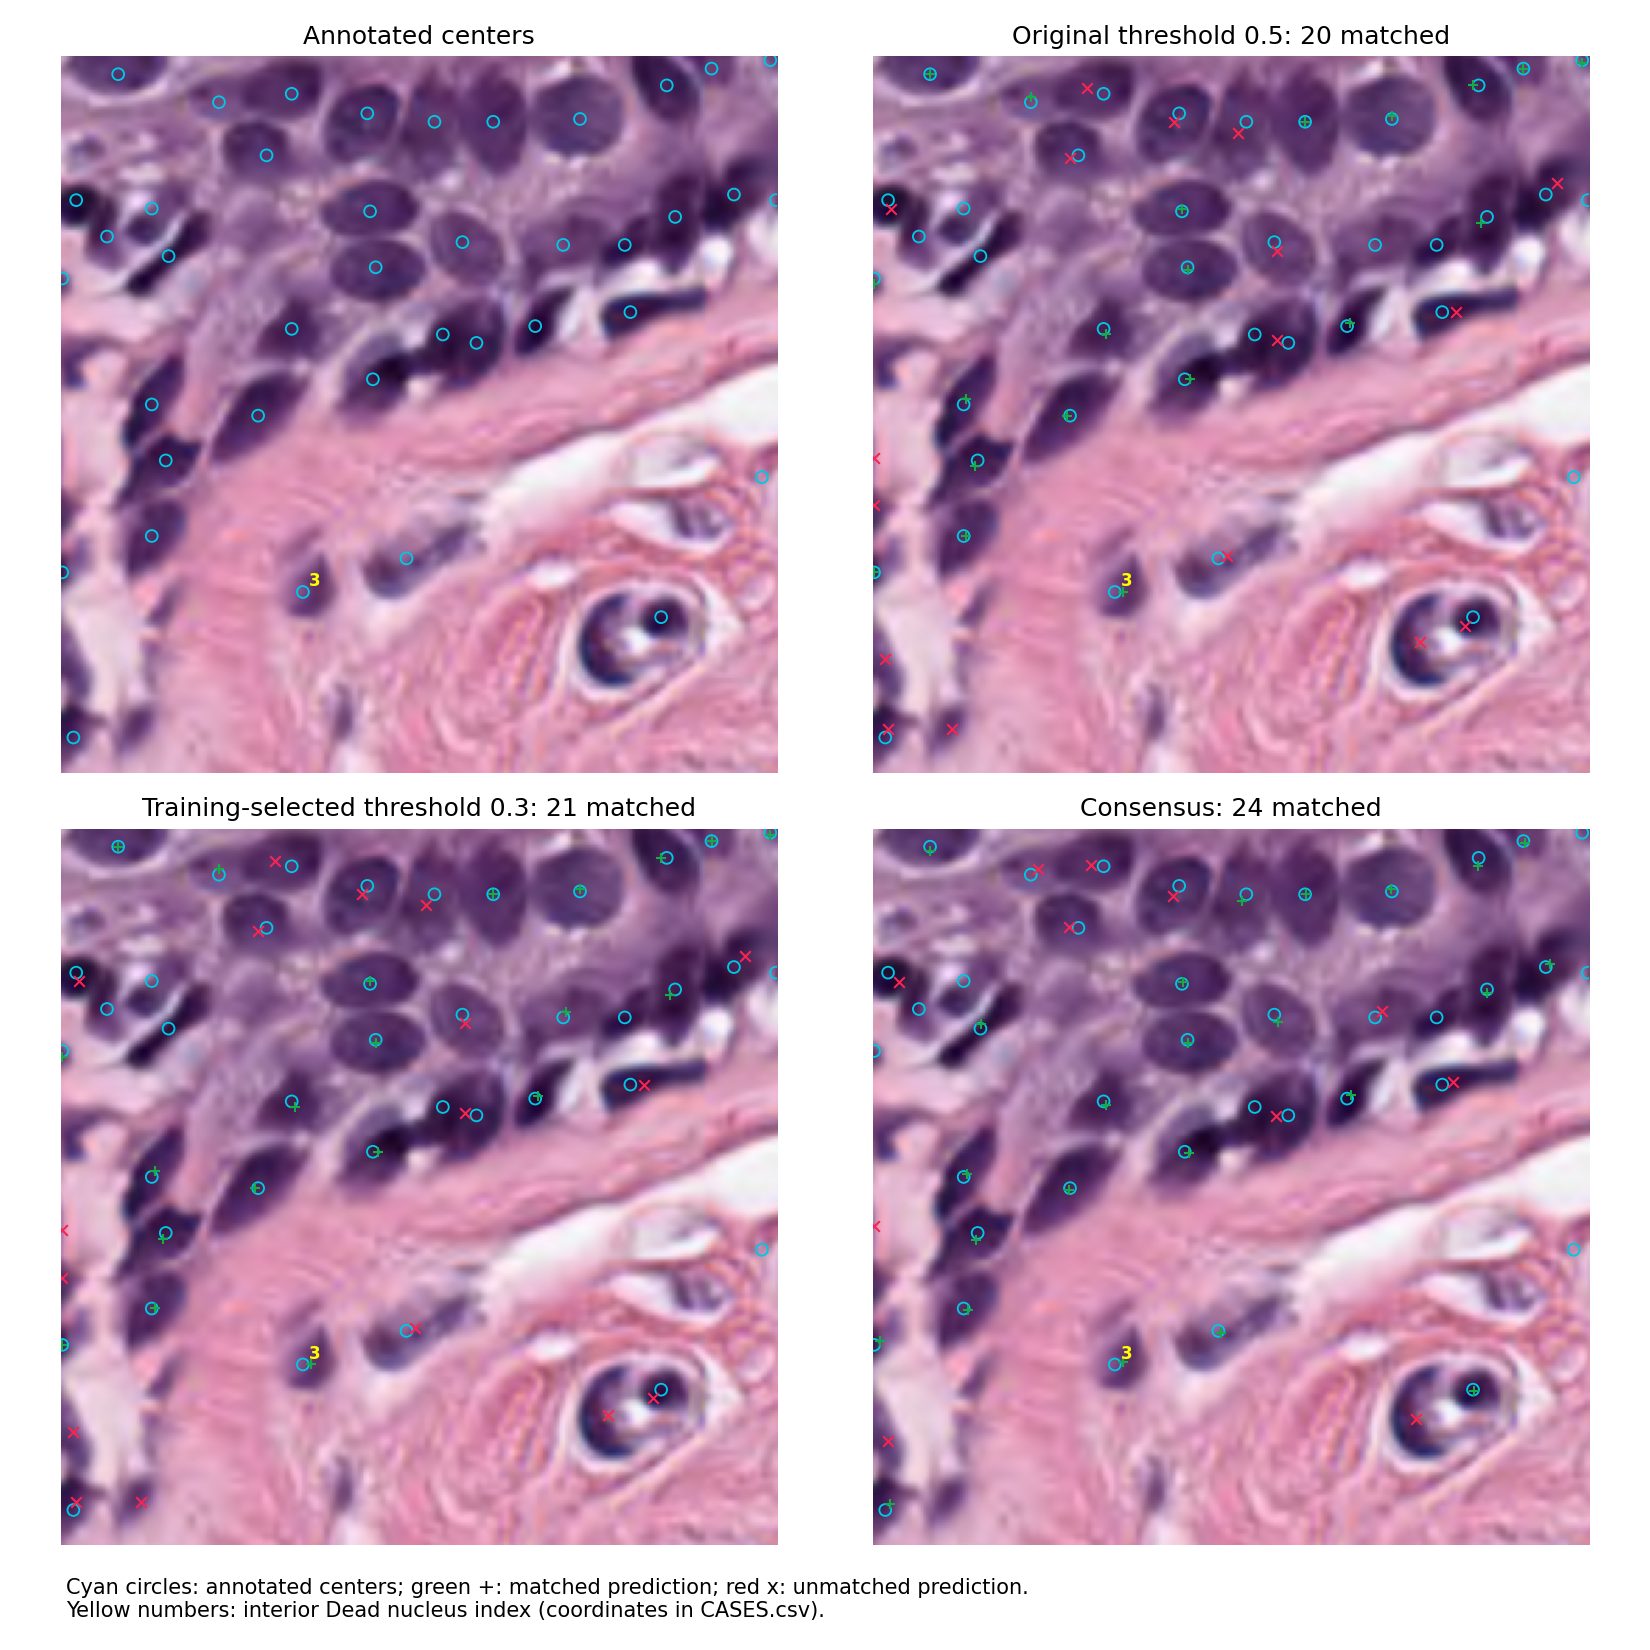
\includegraphics[width=0.9\linewidth,height=\textheight,keepaspectratio,alt={固定乳腺组织图像178，全层适配检测器种子19。}]{assets/P22_M_s19_development_0178.png}
\caption{固定乳腺组织图像178，全层适配检测器种子19。}
\end{figure}

编号23是中心(y,x)=(71,38)的上皮细胞核。原对齐三像素内峰值分数0.202，阈值0.5与0.3都不会保留。四种平移对齐能匹配它；汇总点(69.33,38.33)距标注1.70像素，因而找回该核。

内部死亡核3位于(191,86)，面积286像素，三种解码都保留；原峰值分数0.926，汇总位置距中心2.97像素，已接近三像素边界。增加观察既能找回漏检，也可能把有效点推向匹配边界。

\newpage

\section{结肠组织图像1482：分数不足、找回与持续漏检}\label{ux7ed3ux80a0ux7ec4ux7ec7ux56feux50cf1482ux5206ux6570ux4e0dux8db3ux627eux56deux4e0eux6301ux7eedux6f0fux68c0}

这里使用平移训练检测器种子19。原阈值0.5匹配12个核，选定0.2后匹配26个，一致性汇总匹配18个。中央组织带包含多个相邻的小核，完整坐标与分配记录一并保留。

\begin{figure}
\centering
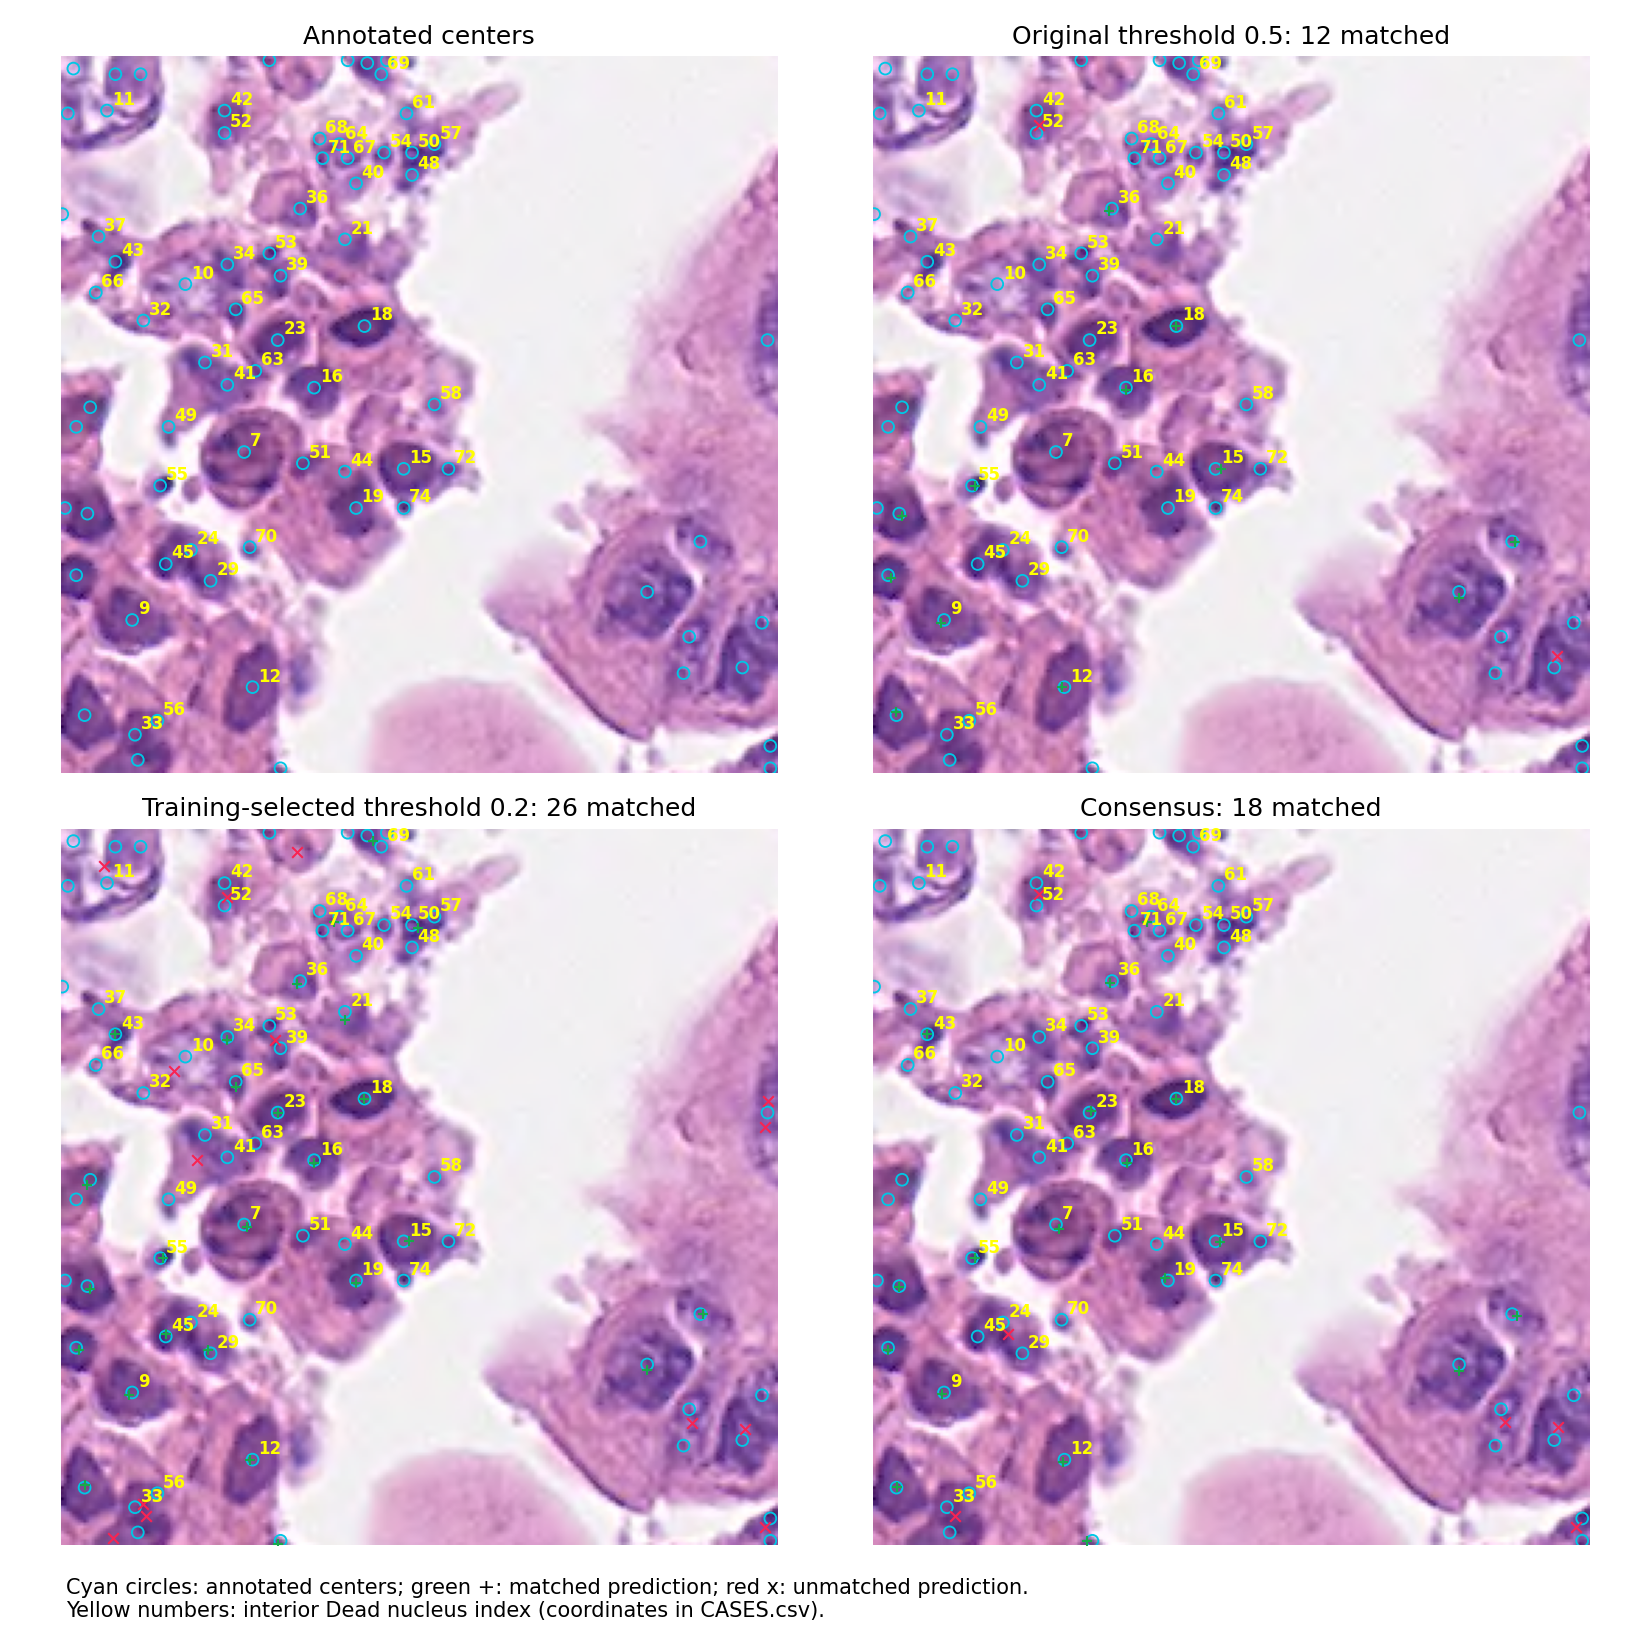
\includegraphics[width=0.9\linewidth,height=\textheight,keepaspectratio,alt={固定结肠组织图像1482，平移训练检测器种子19。}]{assets/P15_J_s19_development_1482.png}
\caption{固定结肠组织图像1482，平移训练检测器种子19。}
\end{figure}

死亡核7位于(141,65)，面积504像素。原对齐中心三像素内的峰值分数0.486，被0.5排除、被0.2保留；十二种平移对齐匹配它，汇总点距中心1.90像素。这颗核同时体现了分数阈值与对齐变化对找回的作用。

死亡核51位于(145,86)，面积67像素，两个检测器均持续漏检。原对齐六像素内没有分数不低于0.1的已记录峰，所有对齐在0.1下也没有三像素内匹配点。附近面积57像素的核55位于(153,35)，却被平移训练模型找到：分数0.575，汇总距离1.11像素；全层模型漏检。小面积与总体困难相关，单颗核的结果还取决于其他图像与模型因素。

\newpage

\section{D37：把剩余漏检分为互斥的五类}\label{d37ux628aux5269ux4f59ux6f0fux68c0ux5206ux4e3aux4e92ux65a5ux7684ux4e94ux7c7b}

本次新增诊断复用P36保存点，没有再次运行检测器。按顺序，每颗核归入：原对齐匹配；原对齐漏检但换对齐在0.5下匹配；只有接纳至0.1的低分数点后匹配；附近点被分给另一颗核；任何对齐在0.1下都没有三像素内预测点。两种填充、两种数据角色均统计。降低阈值可能改变相邻核间的一对一分配，因此严格按既定优先顺序分类。

全层种子19原漏检4271个，其中2476个（58.0\%）换白色填充对齐即可在0.5匹配，401个（9.4\%）只在低分数下匹配，2个涉及分配竞争，1392个（32.6\%）无三像素内已记录点。平移训练种子19原漏检7479个，其中2104个（28.1\%）换对齐可匹配，4141个（55.4\%）需要低分数点，1234个（16.5\%）无三像素内已记录点；种子1重复了这一差异。

下面的中心区域图排除了边缘条带。``某一种对齐有匹配点''利用标注判断点是否可用，统计对象与实际选定解码不同。低于0.1的点未保存；距中心超过三像素的点，即使在核内，也进入最后一类。

\begin{center}
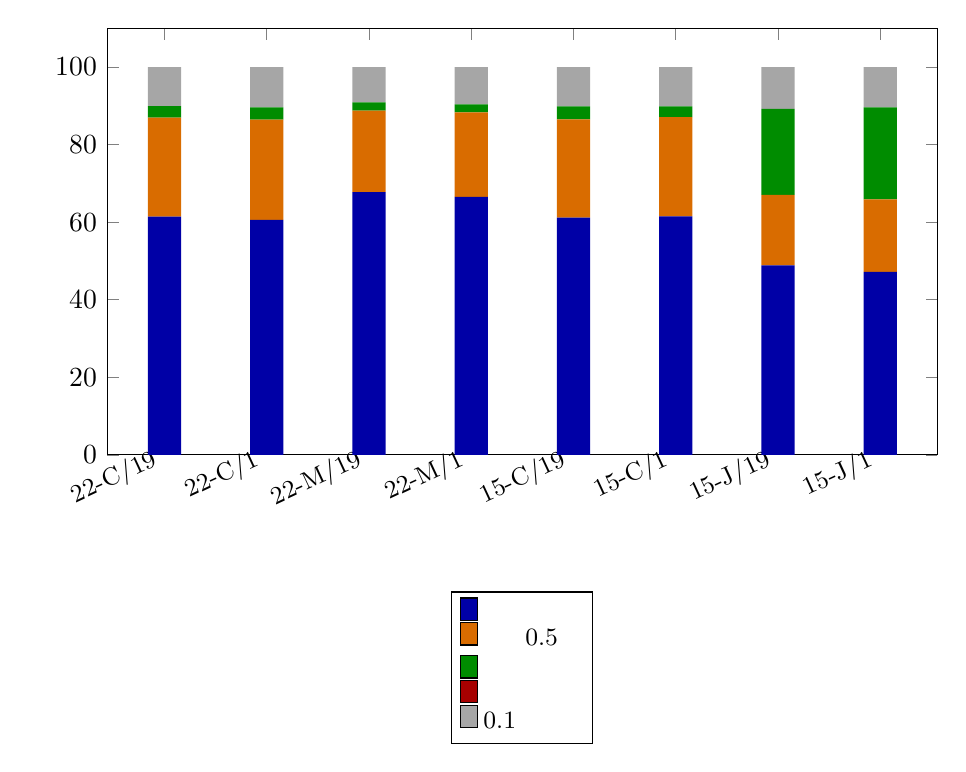
\begin{tikzpicture}
\begin{axis}[width=\linewidth,height=7cm,ymin=0,xtick={0,1,2,3,4,5,6,7},xticklabels={22-C/19,22-C/1,22-M/19,22-M/1,15-C/19,15-C/1,15-J/19,15-J/1},x tick label style={font=\small,rotate=25,anchor=east},ylabel={中心区域标注核（百分比）},legend style={at={(0.5,-0.32)},anchor=north,legend columns=1,font=\small},enlarge x limits=0.08,ybar stacked,bar width=12pt]
\addplot[fill=blue!65!black,draw=none] coordinates {(0,61.448532) (1,60.564585) (2,67.721699) (3,66.524095) (4,61.191902) (5,61.505560) (6,48.873681) (7,47.191332)};
\addplot[fill=orange!85!black,draw=none] coordinates {(0,25.506131) (1,25.862561) (2,21.043627) (3,21.799259) (4,25.320787) (5,25.591674) (6,18.149415) (7,18.676932)};
\addplot[fill=green!55!black,draw=none] coordinates {(0,2.965498) (1,3.136584) (2,2.138580) (3,2.024522) (4,3.321928) (5,2.765897) (6,22.212717) (7,23.709723)};
\addplot[fill=red!65!black,draw=none] coordinates {(0,0.000000) (1,0.000000) (2,0.000000) (3,0.000000) (4,0.000000) (5,0.000000) (6,0.000000) (7,0.000000)};
\addplot[fill=gray!70,draw=none] coordinates {(0,10.079840) (1,10.436270) (2,9.096094) (3,9.652124) (4,10.165384) (5,10.136869) (6,10.764186) (7,10.422013)};
\legend{原对齐匹配,其他对齐在0.5匹配,只在较低分数下匹配,近邻分配竞争,0.1下无三像素内预测点}
\end{axis}
\end{tikzpicture}
\end{center}

7014个中心区域开发评估核的互斥分类，白色填充；下表列出全体核的计数。

\begin{longtable}[]{@{}
  >{\raggedright\arraybackslash}p{(\linewidth - 10\tabcolsep) * \real{0.1304}}
  >{\raggedleft\arraybackslash}p{(\linewidth - 10\tabcolsep) * \real{0.1739}}
  >{\raggedleft\arraybackslash}p{(\linewidth - 10\tabcolsep) * \real{0.1739}}
  >{\raggedleft\arraybackslash}p{(\linewidth - 10\tabcolsep) * \real{0.1739}}
  >{\raggedleft\arraybackslash}p{(\linewidth - 10\tabcolsep) * \real{0.1739}}
  >{\raggedleft\arraybackslash}p{(\linewidth - 10\tabcolsep) * \real{0.1739}}@{}}
\toprule\noalign{}
\begin{minipage}[b]{\linewidth}\raggedright
检测器 / 种子
\end{minipage} & \begin{minipage}[b]{\linewidth}\raggedleft
原对齐匹配
\end{minipage} & \begin{minipage}[b]{\linewidth}\raggedleft
换对齐后匹配
\end{minipage} & \begin{minipage}[b]{\linewidth}\raggedleft
仅低分数匹配
\end{minipage} & \begin{minipage}[b]{\linewidth}\raggedleft
分配竞争
\end{minipage} & \begin{minipage}[b]{\linewidth}\raggedleft
无三像素内预测点
\end{minipage} \\
\midrule\noalign{}
\endhead
\bottomrule\noalign{}
\endlastfoot
22-C/19 & 7,255 & 2,875 & 536 & 1 & 1,583 \\
22-C/1 & 7,199 & 2,893 & 521 & 1 & 1,636 \\
22-M/19 & 7,979 & 2,476 & 401 & 2 & 1,392 \\
22-M/1 & 7,933 & 2,493 & 354 & 2 & 1,468 \\
15-C/19 & 7,255 & 2,849 & 574 & 1 & 1,571 \\
15-C/1 & 7,285 & 2,894 & 498 & 1 & 1,572 \\
15-J/19 & 4,771 & 2,104 & 4,141 & 0 & 1,234 \\
15-J/1 & 4,600 & 2,178 & 4,267 & 1 & 1,204 \\
\end{longtable}

\newpage

\section{位置变化：对齐波动减小，共有偏移仍然存在}\label{ux4f4dux7f6eux53d8ux5316ux5bf9ux9f50ux6ce2ux52a8ux51cfux5c0fux5171ux6709ux504fux79fbux4ecdux7136ux5b58ux5728}

对中心区域的孤立核，只统计至少两种平移对齐在六像素内有保留点的对象。镜像填充下，最后12层模型随对齐变化的均方位移约2.04---2.10平方像素，各对齐共有的部分4.29---4.42；全层模型为1.67、1.68与3.78、3.83；平移训练模型为0.62、0.62与3.46、3.40。

相对于自身对照，平移训练让随对齐变化的量减少约70\%，但共有偏移仍更大。平均多个对齐能减小变化，无法去除共同方向的偏移；稳定预测也可能偏离标注中心。

共有部分采用平均位移的平方，减去对齐内样本方差除以可见点数。这是确定性平移上的描述性矩分解，不能直接把偏移归因为组织内容或标注噪声。统计还以存在近邻保留点为条件：平移训练模型约4500个核，其他模型约6300个，模型之间并非同一保留对象集合。

\begin{center}
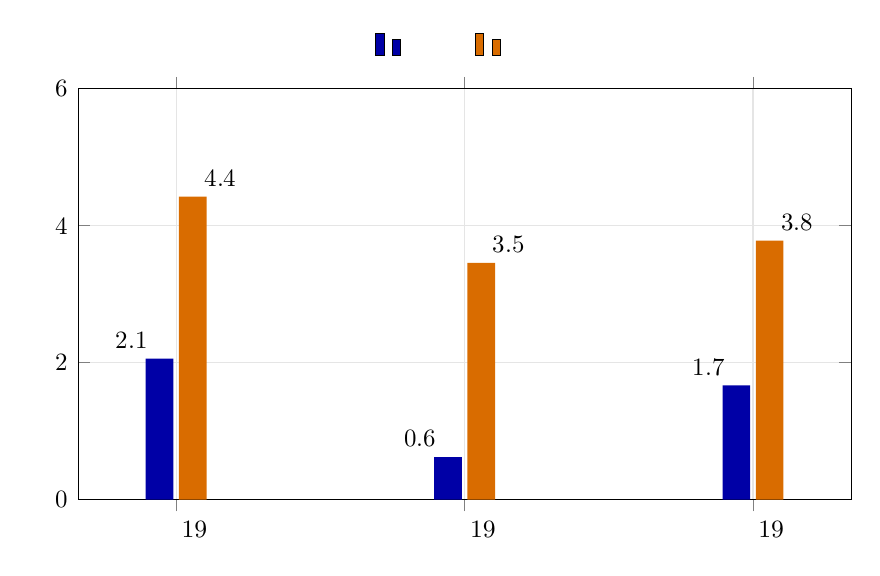
\begin{tikzpicture}
\begin{axis}[width=0.94\linewidth,height=68mm,ybar,bar width=10pt,ymin=0,ymax=6,enlarge x limits=0.17,xtick={0,1,2},xticklabels={{平移对照 19},{平移训练 19},{全层训练 19}},ylabel={平方像素；镜像填充},tick label style={font=\small},label style={font=\small},legend style={at={(0.5,1.06)},anchor=south,legend columns=2,column sep=5pt,draw=none,font=\small},grid=major,major grid style={gray!20}]
\addplot[fill=blue!65!black,draw=none,nodes near coords,nodes near coords style={font=\small,xshift=-10pt,/pgf/number format/fixed,/pgf/number format/precision=1}] coordinates {(0,2.05746077) (1,0.62138397) (2,1.66686793)};
\addplot[fill=orange!85!black,draw=none,nodes near coords,nodes near coords style={font=\small,xshift=10pt,/pgf/number format/fixed,/pgf/number format/precision=1}] coordinates {(0,4.42344983) (1,3.45747238) (2,3.78247919)};
\legend{{随对齐变化},{共有部分}}
\end{axis}
\end{tikzpicture}

\end{center}

开发评估图像、镜像填充，所有检测器使用相同半径、孤立规则与估计式；保留对象集合的差异已在正文交代。

\newpage

\section{研究决策、复现与剩余事项}\label{ux7814ux7a76ux51b3ux7b56ux590dux73b0ux4e0eux5269ux4f59ux4e8bux9879}

当前证据区分了三个环节。第一，全层检测器的许多漏检可通过改变对齐找回，汇总预测位置比直接平均窄分数峰更合适。第二，平移训练减小对齐变化，同时使分数偏低，评估该配置需要把解码校准一并考虑。第三，全层与平移训练模型仍有约9\%---10\%的中心区域开发评估核，在0.1记录下限及所有对齐下没有三像素内预测点；下一步应围绕这些对象的真实图像与分数展开，小核和拥挤核是明确的分层对象。

下一项方法实验应把训练集选择的分数校准与位置支持相结合：P36已为单图解码选低阈值，但一致性汇总仍从0.5起步。独立冻结设计应比较``校准低分数点后再做位置汇总''与现有P36规则，按图像划开训练校准子集，只在训练侧选择参数，保留两种子、最后检查点与原开发评估条件。开发评估曲线中的描述性最优点不进入部署。本任务没有新的检测器训练、掩码扩展或测试折评估。

D37的代码与固定设计在计算前提交。首轮重放漏掉了对象表中没有标注的图像；已加行为回归并在新目录重放，保留这些图像上的额外点。失败输出与日志保留。最终专项验证33项通过，包含既有对齐行为；D37逐图重放八个模型、240张训练和522张开发评估图像的三种解码。源码、摘要、完整对象记录、八张固定样例、测量分数与构建方法均已保存。

P34全层种子1的完整评估、既有大检查点的独立外部归档仍是记录中的待办。P34后续补齐需独立恢复设计与资源核验。最新GPU账目与此前快照不同，本任务使用CPU保存点分析并记录这一不确定性。报告PDF由附带LaTeX源码编译，统计图通过PGFPlots生成，真实组织图像作为原始结果证据嵌入。

\end{document}
